\chapter{Emulace počítačového systému}

Emulace představuje proces, při němž jeden systém (\textbf{hostitelský systém}) napodobuje
architekturu a chování jiného systému (\textbf{cílový systém}). Cílem není pouze spuštění
programu, ale zachování jeho pozorovatelného chování tak, aby software původně určený pro cílovou
architekturu fungoval bez modifikací (binární kompatibilita). Emulace tedy realizuje instrukční
sadu, stav procesoru, paměťový model i komunikaci s periferiemi systému.

Prostředí, ve kterém je napodobovaná architektura, se
nazývá \textbf{emulátorem}. Emulátor může být realizován jak softwarově (program), tak i hardwarově
(FPGA nebo obvod z logických hradel). Tato kapitola bude rozebírat primárně softwarový přístup.

% \section{Emulace, simulace a virtualizace}
%
% V odborné literatuře se často zaměňují pojmy emulace, simulace a virtualizace. Pro účely této práce
% je nutné tyto pojmy přesně vymezit:
%
% \begin{itemize}
%     \item \textbf{Simulace} nemusí zachovávat binární kompatibilitu ani vnitřní implementační
%         detaily, důležitá je věrnost modelovaného jevu.
%     \item \textbf{Virtualizace} je technika používaná tehdy, když hostitelská a cílová architektura
%         jsou shodné. Instrukce mohou být vykonávány přímo fyzickým procesorem a virtualizační vrstva
%         pouze zajišťuje izolaci a řízení přístupu ke zdrojům. U emulace odlišných architektur tento
%         přístup nelze použít.
% \end{itemize}

\section{Úroveň abstrakce a přesnost}

Při návrhu emulátoru je nutné rozhodnout, na jaké úrovni abstrakce bude cílový systém modelován.
Obecně lze rozlišit dva základní přístupy:\cite{emu-wiki-hle-lle}

\begin{itemize}
    \item \textbf{Vysokoúrovňová emulace} (\textit{High-Level Emulation -- HLE}) -- soustředí se na
        reprodukci funkčního chování systému, často bez přesného modelování jednotlivých
        komponentů. Některé operace mohou být nahrazeny přímým voláním funkcí
        hostitelského systému. Tento přístup je obvykle rychlejší, ale může vést k omezené
        přesností a~kompatibilitě.

    \item \textbf{Nízkoúrovňová emulace} (\textit{Low-Level Emulation -- LLE}) -- snaží se modelovat
        architekturu co nejvěrněji, včetně registrů, instrukční sady, paměťové mapy a časování.
        Tento přístup je výpočetně náročnější, ale poskytuje vyšší přesnost a kompatibilitu.
\end{itemize}

Přesnost emulace vyjadřuje do jaké míry emulátor napodobuje chování původní architektury.
Základním kritériem správnosti emulátoru je zachování pozorovatelného chování systému,
tedy reakce na vstupy a generované výstupy. Emulátor lze považovat za správný tehdy, pokud pro
každou posloupnost vstupů produkuje stejnou posloupnost výstupů jako původní systém. To zahrnuje
nejen logickou správnost instrukcí, ale často i jejich časové vztahy.

Vyšší úroveň přesnosti znamená vyšší nároky na výkon hostitelského systému. Obvykle méně přesné
emulátory preferují výkon hostitelského systému a jednoduchost návrhu. Vice přesné emulátory
preferují přesnost emulace cenou výkonu. Emulátory střední přesnosti představují zlatou střední mezi
nízkou a vysokou přesnosti.

\section{Skutečný čas a emulovaný čas}

Pro dosažení precizní synchronizace zavedeme koncept cyklové osy, na které
jsou vyneseny všechny emulované komponenty systému. Tato osa představuje společné
měřítko, kde každý bod odpovídá konkrétnímu stavu všech subsystémů současně, přičemž
její jednotkou jsou synchronizační body. V těchto bodech dochází k předání řízení mezi
jednotlivými komponentami; jeden komponent vykonávání pozastaví a navazuje na něj další,
tak aby byl zachován správný sled operací.

Díky tomu lze přesně modelovat vzájemné interakce, například moment, kdy grafický čip
přistupuje ke sdílené paměti v přesně definovaném cyklu procesoru. Emulátor tak nepracuje
s reálným časem, ale s ,,virtuálními tiky'', které zaručují, že operace proběhnou ve stejném
pořadí a se stejným relativním časováním jako na originálním hardwaru.

\section{Metoda dohánění (catch-up)}
\label{tp:catch-up}

Hlavní výzvou při návrhu emulátoru je transformace přirozeně paralelního chování hardwarových čipů
do sekvenčního kódu hostitelského systému. Na platformách s omezenými zdroji, jako je mikrokontrolér
RP2350, se paralelní či událostní modely ukazují jako neefektivní kvůli vysoké režii synchronizace a
složitosti implementace. Jako optimální řešení se proto jeví sekvenční metoda dohánění
(\textit{catch-up}), která využívá jeden komponent (nejčastěji CPU) jako časovou referenci. Ostatní
části systému pak simulují svůj stav dávkově až ve chvíli, kdy potřebují „dohnat“ počet cyklů
vykonaných tímto opěrným prvkem (obr. \ref{fig:emu_cycle_axis}), což zajišťuje vysoký výkon při
zachování nezbytné věrnosti simulace.

\begin{figure}[htbp]
    \centering
    \includesvg[width=\textwidth]{images/emu_cycle_axis.svg}
    \caption{Znázornění catch-up mechanismu na cyklové ose.}
    \label{fig:emu_cycle_axis}
\end{figure}

Kód \ref{code:sequential-emulator-loop} demonstruje příklad těla smyčky sekvenčního emulátoru,
emulujícího abstraktní systém, který se skládá z CPU a $n$ komponentů. Na začátku cyklu emulátoru se
určí počet cyklů, které má dosáhnout CPU (\ci{cycles\_to\_execute}). Když CPU dokončí vykonávání,
následně všechny komponenty musí dohnat stav odpovídající současnému stavu CPU. Funkce \ci{Sync()}
zajišťuje synchronizovaný a stabilní běh emulátoru (např. podle obnovovací frekvence monitoru).

Počet cyklů, které musí dosáhnout CPU, může být libovolný, ale mohou existovat určité faktory, podle
kterých se dá určit optimální hodnota. Např. u systému, kde určitý komponent může vygenerovat
přerušení, CPU by měl zastavit těsně před nebo přesně v tom cyklu, kdy má dojít k registraci
přerušení procesorem.


\begin{code}[H]
    \begin{algorithmic}
        \WhileNot {$quit$}
            \State $cycles\_to\_execute \gets cpu.cycles + \dots$

            \While {$cpu.cycles < cycles\_to\_execute$}
                \State CpuStep()
            \EndWhile

            \State C1RunUntil($cpu.cycles \ast C1\_CYCLES$)
            \State C2RunUntil($cpu.cycles \ast C2\_CYCLES$)

            \dots

            \State C$n$RunUntil($cpu.cycles \ast Cn\_CYCLES$)

            \State Sync()
        \EndWhile
    \end{algorithmic}
    \caption{Konceptuální realizace metody dohánění (\textit{catch-up}) pro více-komponentní systém.}
    \label{code:sequential-emulator-loop}
\end{code}

Důležitým je, aby žádný z komponentů nepředběhl CPU, a ani nezaostal, jinak to může způsobit
desynchronizaci celého systému nebo jeho části. Synchronizačním bodem musí být striktně současný
bod CPU na cyklové ose.

Funkce \ci{CpuStep()} vykoná jednu instrukci, aktualizuje stav CPU a posune ho po časové ose. Každý
$n$-tý komponent má funkcí \ci{C$n$RunUntil()}, která aktualizuje stav tohoto komponentu a také ho
posune po cyklové ose.

\begin{figure}[H]
    \centering
    \includesvg[width=\textwidth]{images/emu_cycle_axis_on_demand.svg}
    \caption{Znázornění dohánění na požadavek.}
    \label{fig:emu_cycle_axis_on_demand}
\end{figure}

Emulované komponenty také mají dohánět, když CPU k ním přistupuje, a přitom CPU ještě nevykonal
potřebný počet cyklů. Toto rozšíření catch-up mechanismu se nazývá \textit{catch-up on demand} --
dohánění na požadavek (obr. \ref{fig:emu_cycle_axis_on_demand}).

\section{Emulace CPU}

Při emulaci CPU hlavním zájmem je emulace výsledku instrukcí a vnějšího chování procesoru.
Komplexnější procesory, které mohou obsahovat složitý pipeline, připravovat instrukce napřed apod.
obvykle se neemuluje.

Nejjednodušší a nejrozšířenější způsob emulace CPU je \textbf{interpret}. Spočívá v přímé emulaci
instrukčního cyklu (\textit{fetch-decode-execute}) Interpret čte instrukci z paměti a následně ji
dekóduje -- určuje adresovací režimy, případně další informace, a vypočítává adresu kde je uchován
operand. Pak je instrukce přímo vykonána (kód \ref{fig:sequential_emulator_loop}).\cite{bario2001}

\begin{code}
    \begin{algorithmic}
        \Procedure{CpuStep}{}
            \While{$cycles < target\_cycles$}
                \State $opcode \gets $ Fetch()
                \LeftComment{Způsob dekódování instrukcí závisí na emulované architektuře.}
                \State $op\_addr \gets $ Decode($opcode$)
                \State $cycles \gets cycles\ + $ Exec($opcode$, $op\_addr$)
            \EndWhile
        \EndProcedure
    \Procedure{Fetch}{}
        \State $opcode \gets$ memory[PC]
        \State $\text{PC} \gets \text{PC} + 1$
        \State \Return $opcode$
    \EndProcedure
    \Procedure{Exec}{$opcode, op\_addr$}
        \LeftComment{Každá instrukce má přiřazenou implementační funkci.}
        \State $instr \gets$ instr\_table[$opcode$]
        \State $cycles \gets instr(op\_addr)$
        \State \Return $cycles$
    \EndProcedure
    \end{algorithmic}
    \caption{Emulace CPU pomoci interpretu.}
    \label{fig:sequential_emulator_loop}
\end{code}

Nevýhodou této metody je relativně nižší výkon. Každá instrukce musí být nejprve načtená z paměti,
následně dekódována a až poté vykonána odpovídající obslužnou rutinou. Tento proces vyžaduje několik
operací hostitelského procesoru pro vykonání jediné instrukce emulovaného systému. Ve výsledku
emulace může být řádově pomalejší než nativní běh programu na původní architektuře.

Výhodou je jednoduchost implementace (v jazycích odvozených od C obvykle postačí jazyková konstrukce
\ci{switch} nebo tabulka ukazatelů na funkce). Navíc výsledný kód je snadno přenositelný mezi
různými hostitelskými systémy.

Alternativní cestou emulace CPU je dynamická rekompilace (JIT -- \textit{Just-In-Time compilation}),
což je způsob, když emulátor překládá bloky instrukcí emulovaného procesoru do nativního kódu
hostitelské architektury. Tento přístup může výrazně zvýšit výkon emulace, ovšem je mnohem
složitější v implementaci, a u relativně jednoduchých architektur jako 6502 se nevyplatí, proto
nebude rozebírán v této práci.

\section{Emulace pamětí a sběrnice}

Sběrnice a paměť tvoří komunikační páteř systému, která v kontextu emulace nepředstavuje fyzické
vodiče, ale logickou vrstvu řídící veškerý tok informací. Zatímco u nejjednodušších architektur lze
paměť reprezentovat jako prosté lineární pole přístupné přímým indexováním, u komplexnějších
systémů, poskytujících pokročilé funkce nebo přístup k periferiím, není adresní prostor homogenní,
jelikož se zde aplikuje paměťové mapování – technika, při níž jsou konkrétní adresní rozsahy pevně
přiřazeny různým hardwarovým entitám, jako jsou moduly RAM a ROM nebo specifické registry periferií.

\begin{figure}[H]
    \centering
    \includesvg[width=0.75\textwidth]{images/memory_map.svg}
    \caption{Příklad mapované pamětí: adresový prostor CPU systému NES.}
    \label{fig:memory_map}
\end{figure}

Emulovaná sběrnice tak funguje jako dispečer, který zachytává každý požadavek procesoru na
čtení či zápis a na základě definované paměťové mapy jej přesměruje k příslušnému datovému zdroji
nebo k obslužné funkci konkrétního hardwaru. Vzhledem k tomu, že k paměti se přistupuje prakticky v
každém hodinovém cyklu (zejména u Von Neumannových architektur), je rychlost tohoto adresového
dekódování kritická pro celkový výkon systému. V praxi se využívají dva základní přístupy:

\begin{enumerate}
    \item \textbf{Rozvětvené rozhodování} -- emulátor testuje adresu proti pevným rozsahům. Tento
            přístup je sice programátorsky jednoduchý, ale při velkém množství periferních zařízení
            vede k vysoké režii z důvodu mnoha logických porovnání.
    \item \textbf{Stránkování a tabulka ukazatelů} -- paměťový prostor je rozdělen na bloky fixní
        velikosti (např. 1~kB nebo 4~kB). Emulátor udržuje tabulku (pole) funkčních ukazatelů nebo
        adres, kde pro každou „stránku“ adresního prostoru existuje přímý odkaz na obslužnou rutinu
        nebo segment paměti. K ní pak přistupuje pomocí bitového posunu $\text{page\_idx} = addr \gg
        shift$.  Tato metoda je výrazně flexibilnější a umožňuje rychlé přesměrování požadavků bez
        složitých podmínek.
\end{enumerate}

\subsection{Přepínání banek}

Staré systémy využívaly techniky přepínání banek k tomu, aby programy mohly adresovat více pamětí,
než to dovolovává šířka adresní sběrnice. Fyzická paměť byla rozdělená menší bloky, z nichž je v
daný okamžik do adresového prostoru CPU zpřístupněná pouze část.

Emulátor v takovém případě uchovává veškerá data v rozsáhlých polích (např. v paměti hostitelského
systému), ale procesoru zpřístupňuje pouze aktivní „okna“. Při přepnutí banky programem nedochází k
fyzickému kopírování dat, ale pouze ke změně ukazatele v tabulce stránek emulované sběrnice na jinou
část paměti.

Příkladem mohou sloužit herní kazety systému NES. Typicky tyto kazety obsahovaly více paměti, než
kolik byl CPU schopen přímo adresovat, a proto využívaly speciální obvody umožňující přepínání
paměťových bank za běhu programu. Díky tomu hry mohly být mnohem rozsáhlejší. Podrobněji o tom bude
popsáno v podkapitole \ref{sec:mappers}.

\subsection{I/O a vedlejší efekty (Side Effects)}

Většina moderních a historických systémů využívá paměťově mapované I/O, kde periferie komunikují s
CPU prostřednictvím specifických adres v paměťovém prostoru. Emulace sběrnice zde funguje jako most.

Klíčovým konceptem jsou tzv. vedlejší efekty při přístupu k paměti:

\begin{itemize}

\item V případě čtení -- přístup na adresu registru periferie může v emulátoru způsobit změnu stavu
    systému (např. vymazání příznaku přerušení nebo posun interního čítače). Pouhý náhled na hodnotu
    tedy mění logický stav stroje.

\item V případě zápisu -- zápis na specifickou adresu neukládá hodnotu do paměti, ale přímo ovlivňuje
    chování hardwaru (např. změnu barvy pixelu nebo spuštění DMA přenosu).

\end{itemize}

Pro každou takovou adresu musí být v emulátoru realizovány funkce čtení a zápisu.

% \subsection{Endianita}
%
% Při emulaci je nezbytné brát v úvahu endianitu, neboli uspořádání bytů. Pokud se endianita
% hostitelského systému (např. Little-Endian u RP2350) liší od emulovaného systému (např. Big-Endian u
% některých procesorů), musí emulátor sběrnice provádět swapování bajtů při každém vícedatovém
% přístupu (např. při čtení 16bitového slova by udělal $x' = (\text{x} \gg 8) \mid ((\text{x}\ \&\
% \text{0xff}) \ll8)$).
%
% Tento proces může při vysoké frekvenci přístupů do paměti znatelně snížit celkový výkon emulace,
% proto je výhodné navrhovat datové struktury emulátoru tak, aby odpovídaly nativnímu uspořádání
% emulovaného hardwaru.

\section{Dlaždicová grafika}

Grafická emulace je obvykle nejnáročnější částí vývoje, neboť vyžaduje přesnou synchronizaci s
procesorem a spotřebovává většinu výpočetního výkonu hostitelského systému. Historické systémy
(8bitové a 16bitové) nepracovaly s moderními GPU API, pracujícími s geometrii a vertexy, ale
spoléhaly na specializované čipy označované jako \textbf{VDP} (\textit{Video Display Processor})
nebo \textbf{PPU} (\textit{Picture Processing Unit}). Tyto jednotky přebíraly zátěž spojenou s
vykreslováním a umožňovaly obejít tehdejší limity kapacity paměti RAM a výkonu CPU.

V rámci této práce bude popsána \textbf{dlaždicová grafika} (\textit{tile-based graphics}), která je
nejrozšířenější technika tvorby 2D grafiky v historických 8bitových i 16bitových architekturách.

\begin{figure}[H]
    \centering
    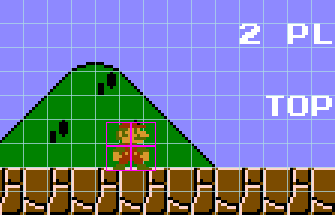
\includegraphics[width=0.5\textwidth]{images/tile_graphics.png}
    \caption{Ukázka dlaždicové grafiky v systému NES: zatímco mřížka pozadí je fixní, mřížka
        jednotlivých spritů se může volně pohybovat. Pořízeno z emulátoru Mesen.}
    \label{fig:tile_graphics}
\end{figure}

Pro úsporu paměti se obraz neskládá z jednotlivých pixelů, ale z mřížky opakovaně použitelných bloků
-- dlaždic (\textit{tile}) o velikosti typicky 8\texttimes8 pixelů. Přitom pixely těchto
dlaždic nejsou skutečné barvy, ale indexy do palet. Vzory dlaždic jsou
uchovány v tabulkách vzorů (\textit{Pattern Table} nebo \textit{Tile Set}). Pro rozmísťování dlaždic
na obrazovce, systém obvykle udržuje mřížku odkazů na tyto vzory (\textit{Nametable} nebo
\textit{Tile Map}). Tento přístup umožňuje efektivní vykreslování rozsáhlých scén a plynulý posun
obrazu (\textit{scrolling}) pouhou změnou hodnot v hardwarových registrech (systémy jako NES dokonce
podporují scrolling s přesností na jeden pixel).

Pro vykreslování pohyblivých dlaždic, které mohou překrývat dlaždice pozadí, se používají tzv.
\textbf{sprity} (nebo také objekty). Sprite představuje dvourozměrnou bitmapu, která není vázaná na
mřížku dlaždic a může obsahovat průhledné pixely. V systémech jako NES, SNES a Game Boy na sprite je
vyhrazená speciální paměť, která se nazývá \textbf{OAM} (\textit{object attribute memory}).

\subsection{Softwarové přístupy k vykreslování v emulátoru}

Zatímco původní hardware generoval obraz postupně, v synchronizaci s paprskem CRT monitoru (případně
obnovováním LCD u kapesních konzolí), emulátor běžící na moderním systému musí tento proces
simulovat. V praxi se volí mezi dvěma hlavními přístupy:

\begin{itemize}
    \item \textbf{Snímkové vykreslování (Frame-based rendering)} -- emulátor nechá běžet CPU po
        dobu, která odpovídá hardwarovému vykreslení celého snímku, a následně celý obraz vygeneruje
        najednou. Tato metoda je výpočetně nejméně náročná, ale selhává u her, které mění grafické
        registry mezi řádky.
    \item \textbf{Řádkové vykreslování (Scanline-based rendering)} -- emulace procesoru se střídá s
        emulací grafiky po každém vykresleném horizontálním řádku (scanline). Tento přístup více
        odpovídá chování skutečného hardwaru a poskytuje vyšší přesnost než snímkové vykreslování,
        avšak nepodporuje meziřádkové modifikace (\textit{mid-scanline modifications} neboli také
        tzv. \emph{rastrové efekty}).
    \item \textbf{Dávkové vykreslování (Batch rendering)} -- tento přístup úzce souvisí s catch-up
        metodou: CPU běží plynule dopředu (nebo po $N$ cyklech) bez neustálé synchronizace s
        PPU. Pokud však CPU provede zápis do grafického registru (nebo naopak potřebuje přečíst stav
        grafického čipu), emulátor pozastaví CPU a nechá PPU „dohnat“ ztracený čas (tzv.
        \textit{catch-up} mechanismus). Grafický čip tak dávkově vygeneruje chybějící pixely či
        řádky přesně do okamžiku, kdy k interakci došlo.
    \item \textbf{Vykreslování na úrovni pixelů (Pixel-based / Cycle-accurate rendering)} --
        představuje nejvyšší možnou úroveň emulace. PPU a CPU jsou striktně synchronizovány na
        úrovni jednotlivých hodinových taktů (či dokonce sub-cyklů). Obraz je generován pixel po
        pixelu, což umožňuje bezchybnou simulaci i těch nejkomplexnějších grafických triků (např.
        změna palety uprostřed vykreslování jednoho řádku). Zásadní nevýhodou je velká výpočetní
        náročnost, zejména v případě mikrokontroléru RP2350, který je použit v praktické částí.
\end{itemize}

Pro většinu 8bitových systému postačí dávkové vykreslování (např. NES nebo Game Boy), jelikož
představuje zlatou střední mezi vykreslováním na úrovní pixelů a řádkovým vykreslováním, a má
střední implementační složitost.

\section{Emulace zvuku}

Zvukový výstup představuje z hlediska emulace zcela odlišnou výzvu než grafika. Zatímco u obrazu
lidské oko toleruje drobné odchylky v časování (například zahození jednoho snímku z šedesáti projde
často bez povšimnutí), lidský sluch je poměrně citlivý na jakékoliv výpadky, fázové posuny nebo
nepravidelnosti. Sebemenší chyba v synchronizaci se okamžitě projeví jako nepříjemné praskání
nebo zkreslení.

\subsection{Syntéza zvuku}

Většina historických 8bitových a 16bitových (včetně NESu) počítačových systémů nedisponovala pamětí
ani výkonem pro přehrávání předem nahraných digitálních vzorků. Místo toho využívaly specializované
obvody označované jako \textbf{PSG} (\textit{Programmable Sound Generator}). Tyto obvody fungují na
principu syntézy zvuku v reálném čase. Obsahují sadu hardwarových oscilátorů, které generují
základní vlnové průběhy (čtvercová, trojúhelníková nebo pilovitá vlna) a generátory
pseudonáhodného šumu. CPU pouze zapisuje do registrů PSG parametry, jako jsou frekvence (výška
tónu), hlasitost a střída (\textit{duty cycle}). Zvukový čip pak na základě těchto parametrů
generuje analogový signál.

Kromě PSG, existují také další metody syntézy jako FM, AM. Však v rámci této práce nebudou popsány,
jelikož systém NES obsahoval jenom několik PSG a jeden jednoduchý DPCM kanál.

\subsection{Vzorkovací (sampled) audio}

Nejběžnější metoda pro přehrávaní neperiodických signálu (a to nejen v historických systémech) je
\textbf{PCM} (\textit{pulse-code modulation} -- pulzně kódová modulace) -- signál je v pravidelných
časových intervalech vzorkován a amplituda každého vzorku je kvantována na nejbližší hodnotu v rámci
definovaného digitálního rozsahu (např. 8 bitů nebo 16 bitů). Přičemž každý vzorek nese absolutní
informaci o své hodnotě v daném čase nezávisle na předchozích vzorcích.

\begin{figure}[H]
    \centering
    \includesvg[width=0.5\textwidth]{images/pcm.svg}
    \caption{Znázornění 4bitového PCM: analogový průběh se dělí na diskrétní body.
        Zdroj \cite{pcm}.}
    \label{fig:pcm}
\end{figure}

Zajímavým případem je herní konzole NES, která využívala metodu DPCM (\textit{differential
pulse-code modulation}) pro přehrávání vzorků, a to její 1bitovou variaci. Namísto ukládáni
absolutní hodnoty každého vzorku se ukládá pouze rozdíl (delta) oproti předchozímu vzorku. Pokud je
přečtený bit 1, výstupní úroveň se zvýší. Pokud je bit 0, úroveň se sníží. Zvuková vlna se tak
,,kreslí'' jako posloupnost malých schůdků nahoru a dolů. Díky tomu bylo možné vměstnat srozumitelný
zvuk do zlomku paměti, kterou by vyžadovalo PCM (avšak kvalita zvuku je znatelně horší).

\subsection{Resampling a aliasing}
\label{sub:downsampling}

Historické zvukové čipy byly zpravidla taktovány přímo z hlavního oscilátoru systému, což znamená,
že jejich vnitřní stav se měnil na frekvencích v řádech megahertzů (např. krok oscilátoru proběhl
téměř dva milionkrát za sekundu). Moderní audio zařízení však vyžadují data v mnohem nižších a
standardizovaných vzorkovacích frekvencích, typicky 44,1 kHz nebo 48 kHz. V tomhle případě je
potřeba přiběhnout k \textbf{downsamplingu}, tedy snížení datového toku při zachování
srozumitelnosti (s minimální ztrátou kvality) zvukového výstupu. Jednou z populárních metod
downsamplingu je \textbf{decimace}, která spočívá ve filtraci signálu pomocí dolní propustí
(low-pass filter) a následném výběru $N$-tého vzorku.\cite{dsp101-decim-intrp}
